\documentclass[tikz, border=10pt]{standalone}
\usepackage{pgfplots}
\usepackage[american]{circuitikz}
\usepgfplotslibrary{groupplots}
\pgfplotsset{compat=1.18}

\begin{document}
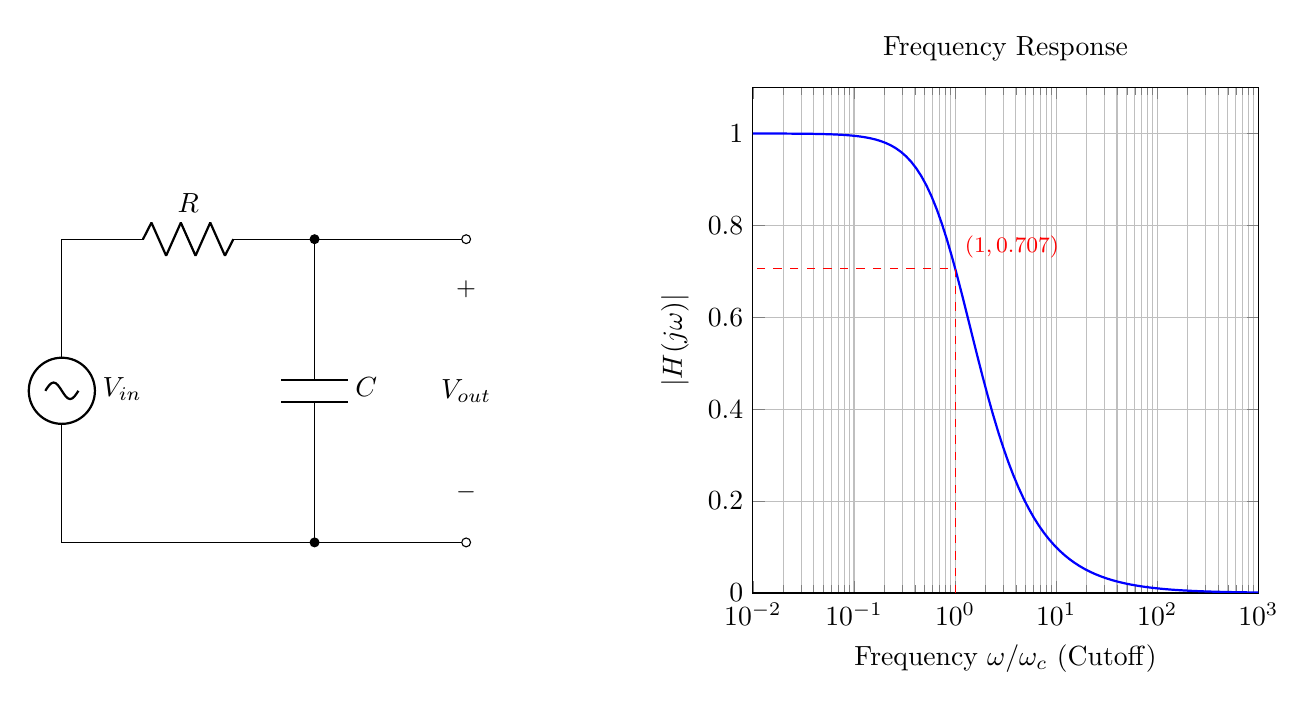
\begin{tikzpicture}
    % Use groupplots to arrange schematic and plot side-by-side
    \begin{groupplot}[
        group style={
            group size=2 by 1,
            horizontal sep=3cm,
        },
        width=8cm, height=8cm,
    ]
    
    % Schematic
    \nextgroupplot[
        axis lines=none,
        xmin=0, xmax=1,
        ymin=0, ymax=1,
    ]
    % Draw circuit inside the first groupplot area
    \draw (axis cs: 0.1, 0.7) to [sV, l=$V_{in}$] (axis cs: 0.1, 0.1)
          to [short] (axis cs: 0.9, 0.1);
    \draw (axis cs: 0.1, 0.7) to [R, l=$R$, -*] (axis cs: 0.6, 0.7)
          to [C, l=$C$, -*] (axis cs: 0.6, 0.1);
    \draw (axis cs: 0.6, 0.7) to [short, -o] (axis cs: 0.9, 0.7);
    \draw (axis cs: 0.6, 0.1) to [short, -o] (axis cs: 0.9, 0.1);
    
    % Vout with polarities
    \node at (axis cs: 0.9, 0.6) {\small $+$};
    \node at (axis cs: 0.9, 0.4) {$V_{out}$};
    \node at (axis cs: 0.9, 0.2) {\small $-$};
    
    % Response Plot
    \nextgroupplot[
        title={Frequency Response},
        xlabel={Frequency $\omega/\omega_c$ (Cutoff)},
        ylabel={$|H(j\omega)|$},
        xmin=0.01, xmax=1000,
        xmode=log,
        ymin=0, ymax=1.1,
        grid=both,
    ]
    % Use log-domain sampling (variable t) for perfectly smooth curves
    \addplot[thick, blue, variable=\t, domain=-2:3, samples=100] ({10^\t}, {1 / sqrt(1 + (10^\t)^2)});
    
    % Mark Cutoff
    \draw[dashed, red] (axis cs: 1, 0) -- (axis cs: 1, 0.707) -- (axis cs: 0.01, 0.707);
    \node[anchor=south west, text=red, font=\footnotesize] at (axis cs: 1, 0.707) {$(1, 0.707)$};

    \end{groupplot}
\end{tikzpicture}
\end{document}
